\begin{frame}
  \frametitle{Model simplification}
  \metroset{block=fill}
  \begin{block}{Why simplification/approximation ? }
  \begin{itemize}
  \item To have a more scalable model (thanks to continuous instead of binary function)
  \item To include duty cycle as a new variable (towards control application)
  \end{itemize}
  \end{block}
  \uncover<2->{
  \begin{block}{Store \& forward method (Aboudolas et al., 2008)}
  Provided that spills are avoided (Demand \&{}Supply paradigm) a flow $f$ becomes
  \begin{columns}[c]
  \column{0.4\textwidth}
  \[
  f = \left\{
  \begin{aligned}
  &0 \mbox{ if } u(t)=0\\
  &\varphi \mbox{ otherwise}
  \end{aligned}
  \right.
  \]  
  \column{0.4\textwidth}
  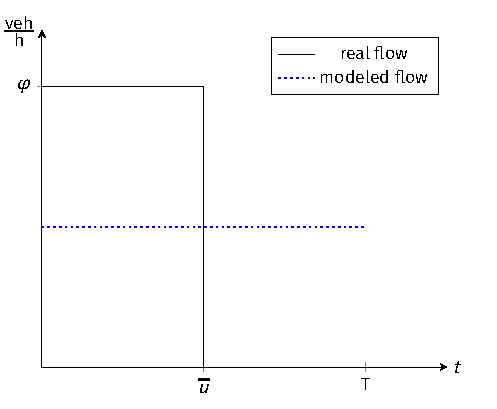
\includegraphics[scale=0.5]{fig_52_SFM}  
  \end{columns}
  \end{block}
  }
\end{frame}